%%%%%%%%%%%%%%%%%%%%%%%%%%%%%%%%%%%%% 
%% LE2I beamer template
%% Guillaume Lemaitre, October 2014
%%%%%%%%%%%%%%%%%%%%%%%%%%%%%%%%%%%%% 

\documentclass{beamer}

\usepackage[utf8]{inputenc}
\usepackage[T1]{fontenc} 
\usetheme{le2i} 

%% The amssymb package provides various useful mathematical symbols
\usepackage{amssymb}
%% The amsthm package provides extended theorem environments
\usepackage{amsthm}
%% amsmath for math environment
\usepackage{amsmath}

\DeclareMathOperator*{\argmin}{arg\,min}
\DeclareMathOperator*{\argmax}{arg\,max}
\DeclareMathOperator*{\sign}{sign}

%% figure package
\usepackage{epsf,graphicx}
\usepackage{epstopdf}
\usepackage{subfigure}
\usepackage{transparent}
\usepackage{caption}
\captionsetup{font=scriptsize,labelfont=scriptsize,labelformat=empty}
\setbeamertemplate{caption}{\raggedright\insertcaption\par}

%% In order to draw some graphs
\usepackage{tikz,xifthen}
\usepackage{tikz-qtree}
\usepackage{adjustbox}
\usetikzlibrary{decorations.pathmorphing}
\usetikzlibrary{fit}
\usetikzlibrary{backgrounds}
\usetikzlibrary{shapes,arrows,shadows}
\usetikzlibrary{calc,decorations.pathreplacing,decorations.markings,positioning}
\usetikzlibrary{snakes,decorations.text,shapes,patterns}
% \usepackage{scalefnt,lmodern,booktabs}

%% Package for cross and tick symbols
\usepackage{pifont}
\newcommand{\tick}{\color{green!60!black!80}\ding{51}}
\newcommand{\cross}{\color{red!60!black!80}\ding{55}}

\usepackage{enumitem}
\setitemize{label=\usebeamerfont*{itemize item}%
  \usebeamercolor[fg]{itemize item}
  \usebeamertemplate{itemize item}}

% \usepackage{apalike}
\usepackage[style=verbose,autocite=footnote,maxnames=10,babel=hyphen,hyperref=true,abbreviate=false,backend=biber,mcite]{biblatex}
\addbibresource{literature_review.bib}
\setbeamertemplate{footnote}{%
  \tiny%
  \parindent 1em\noindent%
  \raggedright
  \hbox to 1.8em{\hfil\insertfootnotemark}\insertfootnotetext\par%
}%
\setlength\footnotesep{0pt}

\title{\Large{Classification of SD-OCT Volumes with LBP: Application to DME Detection}}
\author{\scriptsize{G.~Lema\^itre, M.~Rastgoo, J.~Massich, S.~Shrinivasan, F.~M\'eriaudeau, and D.~Sidib\'e}}
\date{MICCAI-OMIA \\ 9\textsuperscript{th} Oct. 2015}

\institute{Universit\'e de Bourgogne \& Universitat de Girona} 

%% Uncomment if you want to avoid thousand of bullet inside the menu
% \usepackage{etoolbox}
% \makeatletter
% \patchcmd{\slideentry}{\advance\beamer@xpos by1\relax}{}{}{}
% \def\beamer@subsectionentry#1#2#3#4#5{\advance\beamer@xpos by1\relax}%
% \makeatother

\begin{document}

% Show the title page
\begin{frame}
  \titlepage
\end{frame}

% Show the table of contents
\begin{frame}
  \tableofcontents[sectionstyle=show,subsectionstyle=show,subsubsectionstyle=hide]
\end{frame}

\section{Introduction}

\subsection{State-of-the-art}

\section{DME detection}

\subsection{Framework}

\begin{frame}
  \frametitle{DME detection}
  \framesubtitle{Framework}
  \begin{block}{Overview}
    \begin{figure}
      \centering
      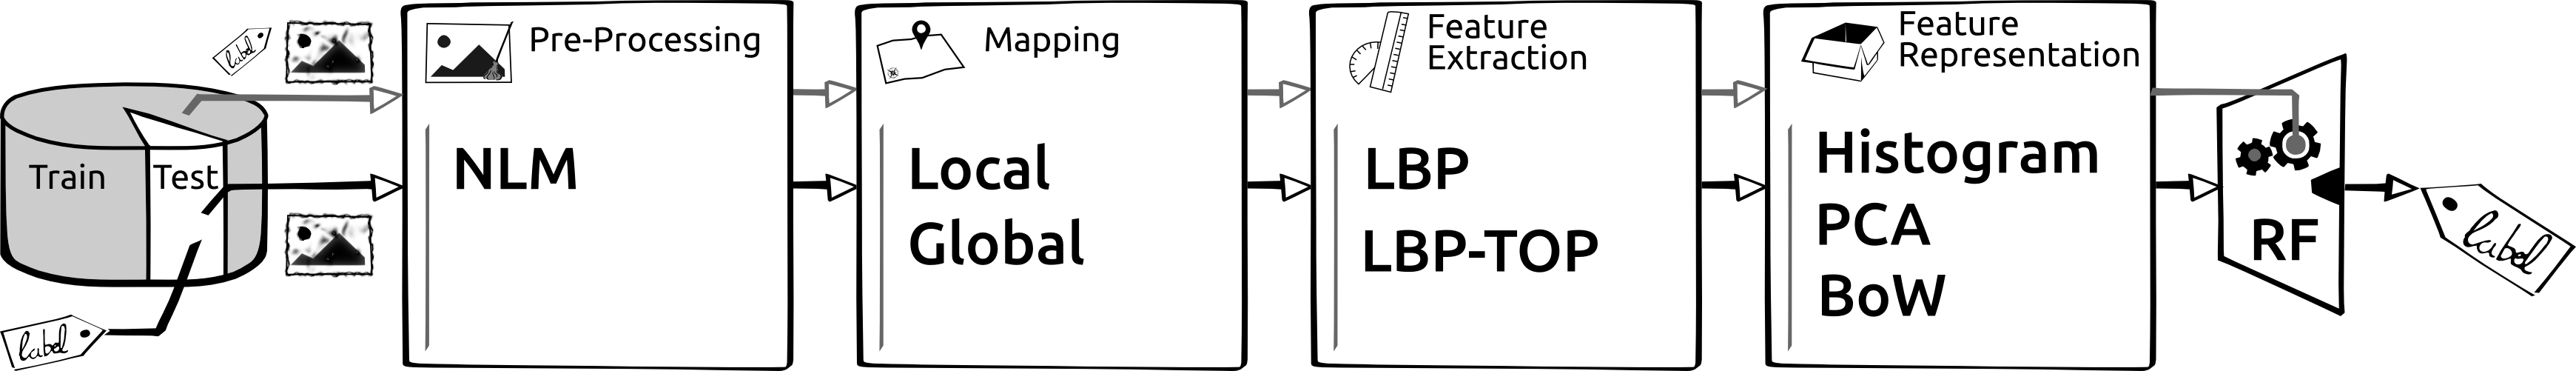
\includegraphics[width=1.\textwidth]{./images/ml.png}
      % \caption{Include an image}
    \end{figure}
  \end{block}
\end{frame}

\subsection{Image pre-processing}

\begin{frame}
  \frametitle{DME detection}
  \framesubtitle{Image pre-processing}
  \begin{block}{Reference system}
    \begin{columns}
      \begin{column}{.3\linewidth}
        \begin{figure}
          \centering
          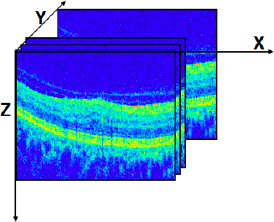
\includegraphics[width=.6\textwidth]{./images/volume.png}
          % \caption{Include an image}
        \end{figure}
      \end{column}
      \begin{column}{.6\linewidth}
        \begin{itemize}[leftmargin=*]\footnotesize
        \item OCT images corrupted with speckle noise
        \item Denoising for each B-scan ($x-z$ slice)
        \item \textbf{Non-Local Means}~\footnotemark
        \end{itemize}
      \end{column}
    \end{columns}
  \end{block}
  \begin{block}{Qualitative results}
    \begin{columns}
      \begin{column}{.5\linewidth}
        \begin{figure}
          \centering
          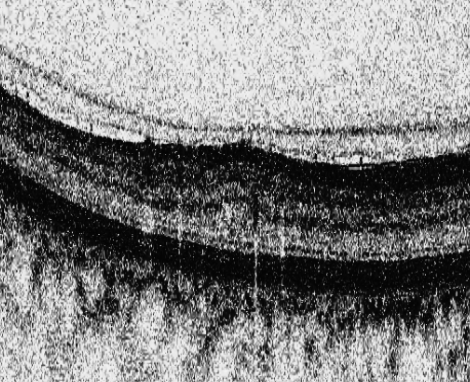
\includegraphics[width=.4\textwidth]{./images/raw_crop_grey.png}
          \caption{Raw image}
        \end{figure}
      \end{column}
      \begin{column}{.5\linewidth}
        \begin{figure}
          \centering
          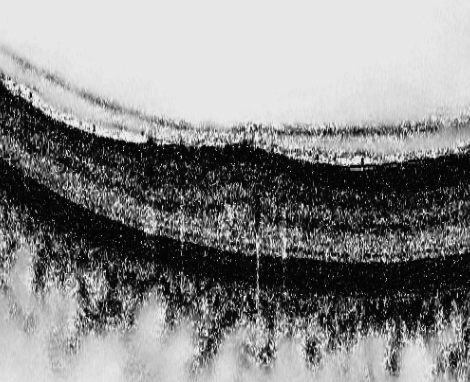
\includegraphics[width=.4\textwidth]{./images/nlm_crop_grey.png}
          \caption{NLM denoising}
        \end{figure}
      \end{column}
    \end{columns}
  \end{block}
  \footcitetext{Coupe2009}
\end{frame}

\subsection{Mapping}

\begin{frame}
  \frametitle{DME Detection}
  \framesubtitle{Mapping}
  \begin{block}{Global mapping}
    \begin{columns}
      \begin{column}{.5\linewidth}
        \begin{figure}
          \centering
          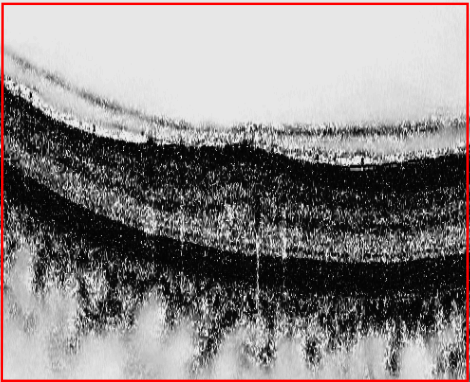
\includegraphics[width=.4\textwidth]{./images/global-2d.png}
          %\caption{Raw image}
        \end{figure}
      \end{column}
      \begin{column}{.5\linewidth}
        \begin{figure}
          \centering
          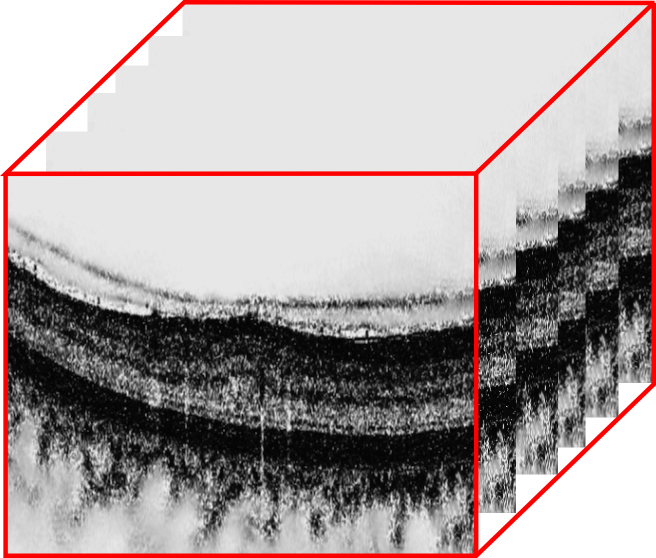
\includegraphics[width=.4\textwidth]{./images/global-3d.png}
          %\caption{NLM denoising}
        \end{figure}
      \end{column}
    \end{columns}
  \end{block}
  \begin{block}{Local mapping}
    \begin{columns}
      \begin{column}{.5\linewidth}
        \begin{figure}
          \centering
          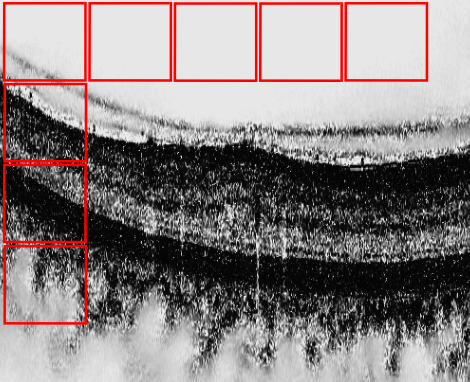
\includegraphics[width=.4\textwidth]{./images/local-2d.png}
          %\caption{Raw image}
        \end{figure}
      \end{column}
      \begin{column}{.5\linewidth}
        \begin{figure}
          \centering
          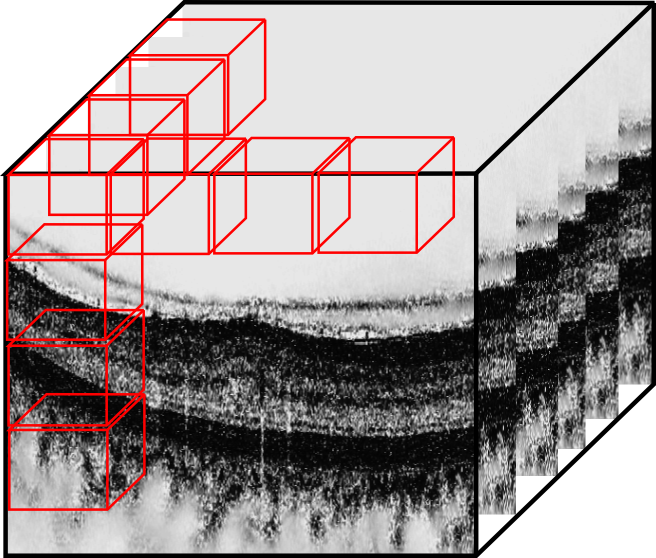
\includegraphics[width=.4\textwidth]{./images/local-3d.png}
          %\caption{NLM denoising}
        \end{figure}
      \end{column}
    \end{columns}
  \end{block}
\end{frame}

\subsection{Local Binary Pattern}

\begin{frame}
  \frametitle{DME Detection}
  \framesubtitle{Local Binary Pattern}
  \begin{block}{LBP}
    \begin{columns}
      \begin{column}{.4\linewidth}
        \begin{figure}
          \centering
          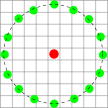
\includegraphics[width=.4\textwidth]{./images/lbp.png}
          %\caption{Raw image}
        \end{figure}
      \end{column}
      \begin{column}{.6\linewidth}
        {\tiny
          \begin{align*}\hspace*{-1cm}
          LBP_{P,R} = \sum_{p=0}^{P-1}s(g_{p} - g_{c})2^{p} \ ,~ s(\cdot) = \begin{cases}                                  
            1  & \ \text{if } (g_{p} - g_{c}) \geq 0\\                                                                         
            0  & \ \text{otherwise}\\                                                                                          
          \end{cases} \ ,                                                                                                        
        \end{align*}}%
      \begin{itemize}[leftmargin=*]\footnotesize
        \item Select uniform and rotation invariant
      \end{itemize}
      \end{column}
    \end{columns}
  \end{block}
  \begin{block}{LBP-Three Orthogonal Plane (TOP)}
    \begin{figure}
      \centering
      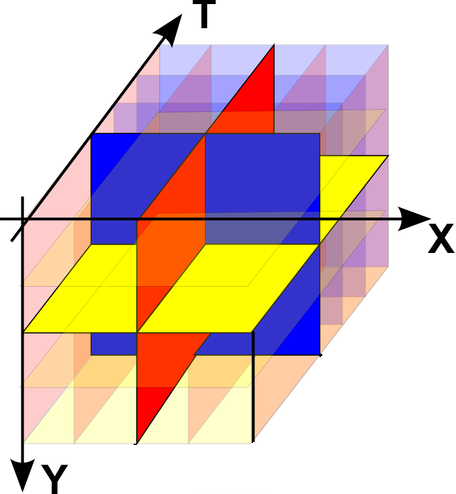
\includegraphics[width=.2\textwidth]{./images/lbp_top.png}
      % \caption{Raw image}
    \end{figure}
  \end{block}
\end{frame}

\subsection{Feature representation}

\begin{frame}
  \frametitle{DME Detection}
  \framesubtitle{Feature representation}
  \begin{block}{Low-level representation}\footnotesize
    \begin{center}
      $\rightarrow$ Compute the histogram of the LBP codes
    \end{center}
    \vspace{-.6cm}
    \begin{columns}
      \begin{column}{.5\linewidth}
        \begin{center}
          Global mapping
        \end{center}
        \begin{description}\footnotesize
          \item[LBP] Concatenation of histogram per B-scan
          \item[LBP-TOP] Concatenation 
        \end{description}
        \begin{itemize}
          \item 1 LBP histogram per B-scan
        \end{itemize}
      \end{column}
      \begin{column}{.5\linewidth}
        \begin{center}
          Local mapping
        \end{center}
        \begin{itemize}
          \item 1 LBP histogram per window
        \end{itemize}
      \end{column}
    \end{columns}
  \end{block}
  \begin{block}{High-level representation}
    \begin{figure}
      \centering
      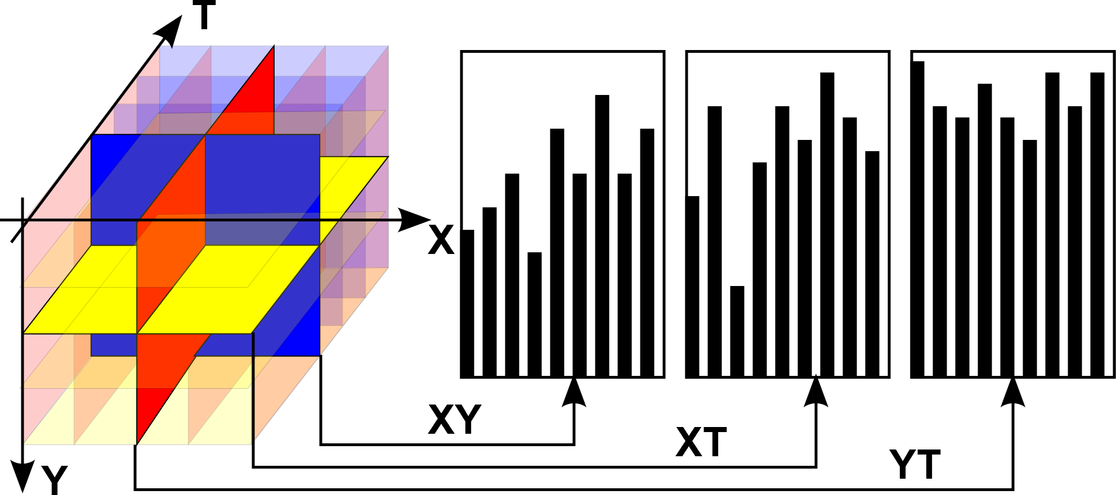
\includegraphics[width=.4\textwidth]{./images/LBPTOP_fig.png}
      % \caption{Raw image}
    \end{figure}
  \end{block}
\end{frame}

%\section*{References}

% \begin{frame}[allowframebreaks]
%   \frametitle{References}
%   \bibliographystyle{apalike}
%   \bibliography{literature_review.bib}
% \end{frame}

% \section{First section}

% \subsection{First subsection}

% \begin{frame}
%   \frametitle{A Kick-Ass Title}
%   \framesubtitle{A Kick-Ass Title Subtitle}
%   \begin{block}{Block environment}
%     \begin{itemize}
%     \item Item 1
%     \item Item 2
%     \end{itemize}
%   \end{block}
%   \begin{figure}
%     \centering
%     \includegraphics[width=.2\textwidth]{./images/logos/le2i-logo.pdf}
%     \caption{Include an image}
%   \end{figure}
% \end{frame}

% \subsection{Second subsection}

% \begin{frame}
%   \frametitle{A Kick-Ass Title}
%   \framesubtitle{A Kick-Ass Title Subtitle}
%   \begin{block}{Block environment}
%     \begin{itemize}
%     \item[\cross] Cross item
%     \item[\tick] Tick item
%     \end{itemize}
%   \end{block}
%   \begin{equation}
%     \label{eq:eq1}
%     f(x)=ax+b \ .
%   \end{equation}
% \end{frame}


\end{document}
%%% Local Variables:
%%% mode: latex
%%% TeX-master: t
%%% End:
